% -*- root: ../ProjectPlan.tex -*-
\section{Time estimation and Schedule}
\label{secTimeEstimation}
\subsection{Gantt diagram}

\begin{figure}[hbtp]
\centering
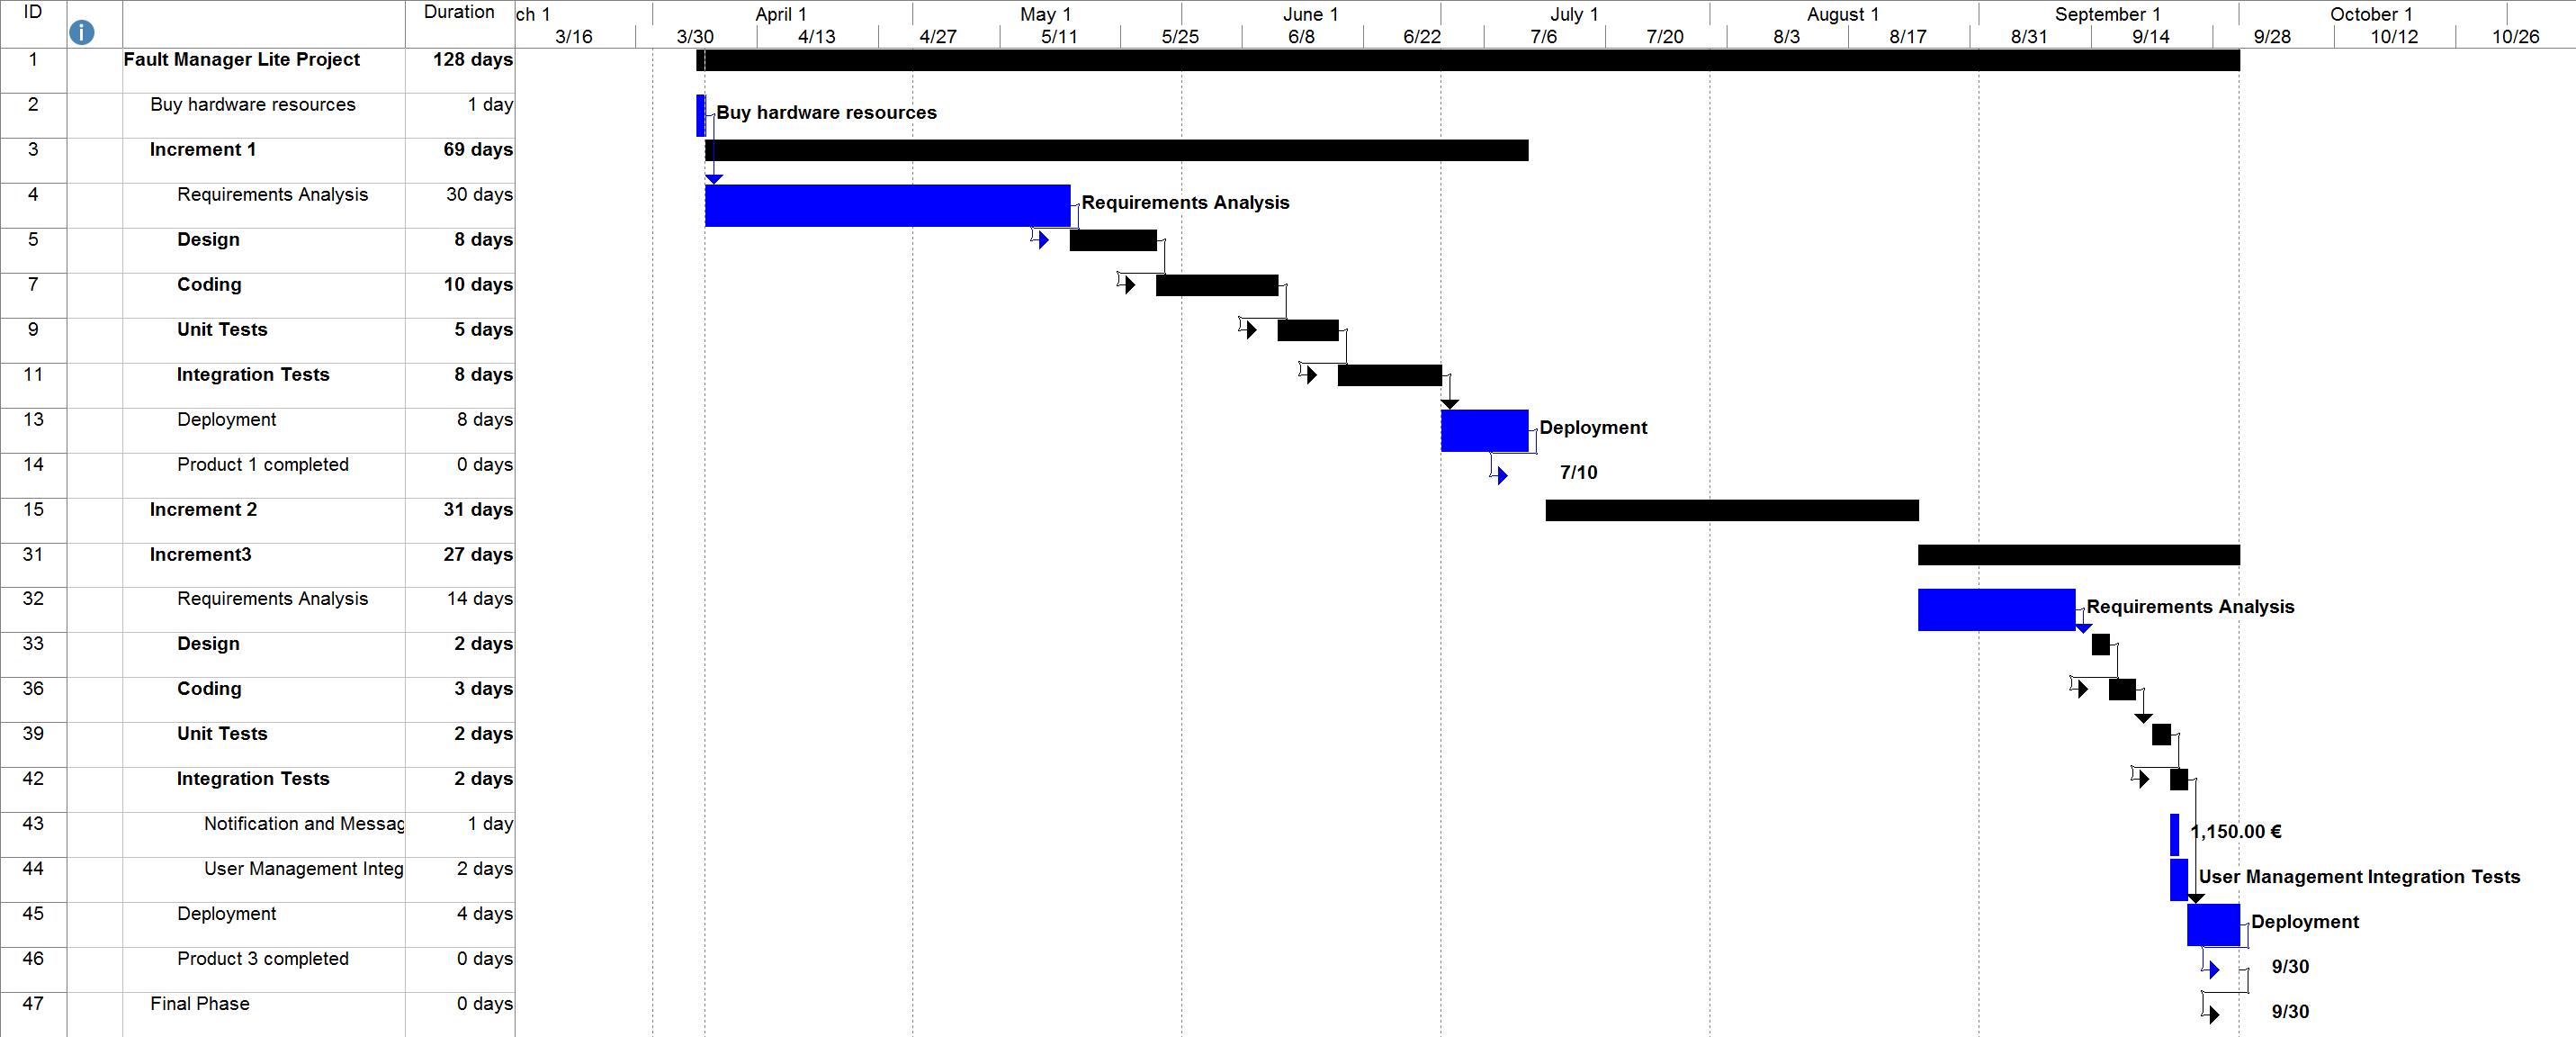
\includegraphics[width=0.8\textwidth]{../GanttDiagram.png}
\caption{Simplified Gantt diagram.}
\label{figGanttSimple}
\end{figure}

Figure \ref{figGanttSimple} shows a simplified view of the Gantt diagram that represents the schedule of the project. A detailed version of this diagram is included in appendix \ref{chapGantt}.

\subsection{Increment planning}

We have decided to break down the development in 3 increments, each one dedicated to various subsystems. The details of the function points assigned to each increment and the corresponding effort is detailed in table \ref{tblIncrementsSubsystems}. Table \ref{tblSubsystemsAssignedIncrement} reflects the increment in which each subsystem will be completed and the corresponding percentage of each increment's effort dedicated to it.

\begin{table}[hbtp]
\centering

\begin{tabular}{c|l|c|c}
\textbf{Increment} & \textbf{Subsystems} & \textbf{Function Points} & \textbf{Effort (person-days)} \\ \hline
Increment 1 & Task management & 102.3 & 149.972 \\
Increment 2 & Report System, Fault History & 50.6 & 74.213 \\
Increment 3 & Notification and Messaging & 48.4 & 70.986 \\ \hline
\textit{Total} &  & \textit{201.3} & \textit{295.106} \\
\end{tabular}

\caption{Detail of the increments and corresponding effort.}
\label{tblIncrementsSubsystems}
\end{table}

\begin{table}[hbtp]
\centering

\begin{tabular}{l|c|c}
\textbf{Subsystem} & \textbf{Increment} & \textbf{Effort \%}  \\ \hline
Task Management & 1 & 100 \% \\
Reporting & 2 & 28 \% \\
Notification and Messaging & 2 & 72 \% \\
User Management & 3 & 36 \% \\
Faults History and Stats & 3 & 64 \% \\
\end{tabular}

\caption{Assigned increment and effort for each subsystem.}
\label{tblSubsystemsAssignedIncrement}
\end{table}

The effort for each phase of each increment is detailed in table \ref{tblIncrementPhases}.

\begin{table}[hbtp]
\centering

\begin{tabular}{|c|c|c|c|}
\hline
\textbf{Increment} & \textbf{Phase} & \textbf{Effort \%} & \textbf{Effort (person-days)} \\ \hline \hline

\multirow{7}{*}{\textsc{Increment 1}} & Analysis & 20 \% & 29.99 \\ \cline{2-4}
& Design & 20 \% & 29.99 \\ \cline{2-4}
& Coding & 20 \% & 29.99 \\ \cline{2-4}
& Unit tests & 10 \% & 14.99 \\ \cline{2-4}
& Integration tests & 20 \% & 29.99 \\ \cline{2-4}
& Implementation & 10 \% & 14.99 \\ \cline{2-4}
& \textit{Total} & \textit{100\%} & \textit{149.972} \\ \hline \hline

\multirow{7}{*}{\textsc{Increment 2}} & Analysis & 20 \% & 14.84 \\ \cline{2-4}
& Design & 20 \% & 14.84 \\ \cline{2-4}
& Coding & 20 \% & 14.84 \\ \cline{2-4}
& Unit tests & 10 \% & 7.42 \\ \cline{2-4}
& Integration tests & 20 \% & 14.84 \\ \cline{2-4}
& Implementation & 10 \% & 7.42 \\ \cline{2-4}
& \textit{Total} & \textit{100\%} & \textit{74.213} \\ \hline \hline

\multirow{7}{*}{\textsc{Increment 2}} & Analysis & 20 \% & 14.2 \\ \cline{2-4}
& Design & 20 \% & 14.2 \\ \cline{2-4}
& Coding & 20 \% & 14.2 \\ \cline{2-4}
& Unit tests & 10 \% & 7.1 \\ \cline{2-4}
& Integration tests & 20 \% & 14.2 \\ \cline{2-4}
& Implementation & 10 \% & 7.1 \\ \cline{2-4}
& \textit{Total} & \textit{100\%} & \textit{70.986} \\ \hline

\end{tabular}

\caption{Detail of the increments with the corresponding phases for each one.}
\label{tblIncrementPhases}
\end{table}
